\documentclass[crop, tikz]{standalone}
\usepackage{tikz}

\usetikzlibrary{calc}
\usepackage{colortbl}

 
 % Definition of circles
\def\square{(-2,-2) rectangle (4,2)}
\def\firstcircle{(0,0) circle (1.5cm)}
\def\secondcircle{(0:2cm) circle (1.5cm)}

\colorlet{circle edge}{black}
\colorlet{circle area}{gray!30!blue!20}

\colorlet{circle edge2}{black!80}
\colorlet{circle area2}{blue}


\tikzset{filled/.style={fill=circle area, draw=circle edge, thick},
	filled2/.style={fill=circle area2, draw=circle edge2, thick},
    outline/.style={draw=circle edge, thick}}

\setlength{\parskip}{5mm}
 
 \begin{document}

 
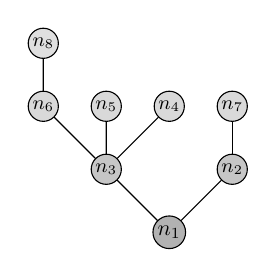
\begin{tikzpicture}[scale=0.8, transform shape, level distance=10mm,
   every node/.style={fill=gray!60,circle,inner sep=1pt},
   level 1/.style={sibling distance=20mm,nodes={fill=gray!45}},
   level 2/.style={sibling distance=10mm,nodes={fill=gray!30}},
   level 3/.style={sibling distance=5mm,nodes={fill=gray!25}}] 
 
  \node[circle,draw]  {$n_1$} [grow=up]
    child {node[circle,draw] {\small $n_2$}
       child {node[circle,draw] {\small $n_7$}}}
    child {node[circle,draw]  {\small $n_3$}
      child {node[circle,draw]  {\small $n_4$}}
      child {node[circle,draw]  {\small $n_5$}}
      child {node[circle,draw]  {\small $n_6$}
         child {node[circle,draw] {\small $n_8$}}}
    };
 

 
 
\end{tikzpicture}
 
\end{document}
